\chapter{PGM Activity after Neutron Irradiation}
\label{section:pgmactivity}

The neutron activity code was used to roughly approximate activities and compare that of 304SS doped with 1\% of the following: Mn, Mo, Pd, Pt and Ru; against an plain sample (Fe 19 Cr 10 Ni).  The simulation was 1MeV neutrons in a Maxwell-Bolztmann distribution for 10 hours of irradiation with 1 hour of cooling.  The activities are relative to one another.  Mn as an additive is known to be a problem element due to the creation of ${}^{56}Mn$ and has been included for comparison.

\begin{figure}
\centering
\begin{minipage}{0.8\textwidth}
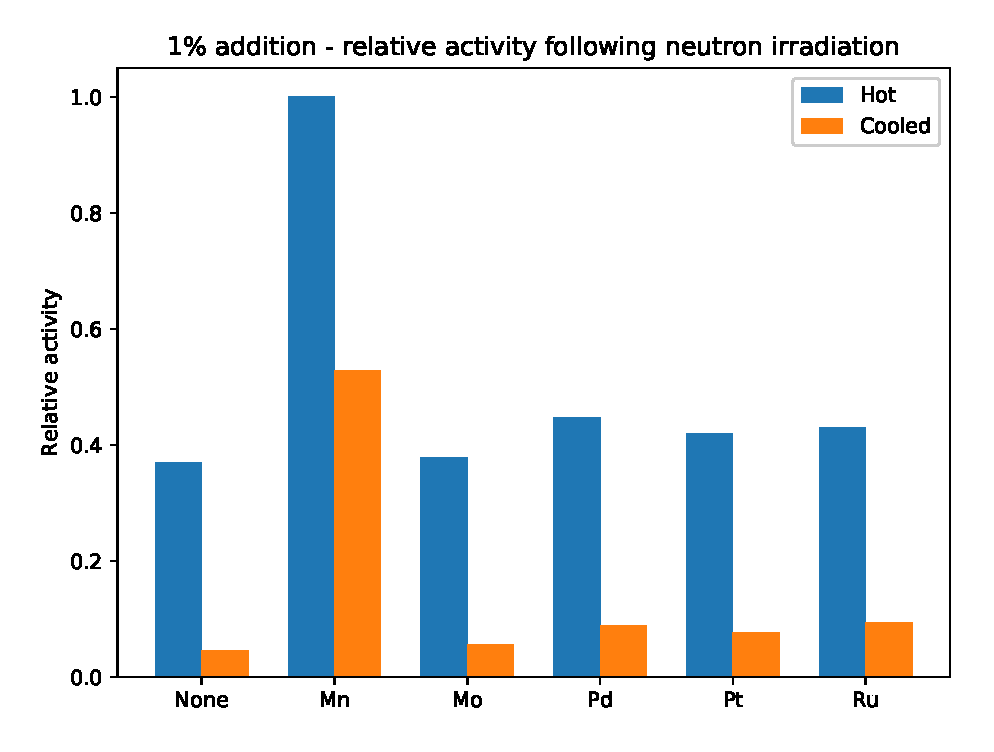
\includegraphics[width=1.0\linewidth]{appendix/pgmactivity/comparitive_activities.eps}
\end{minipage}
\caption{Relative activity hot (just after irrdiation) and cooled (1 hour of cooling) for 1MeV neutron irradiated SS304 and SS304 with 1\% addition of Mn, Mo, Pd, Pt and Ru}
\label{fig:relativeactivitiesSS304}
\end{figure}

\begin{figure}
\centering
\begin{minipage}{.49\textwidth}
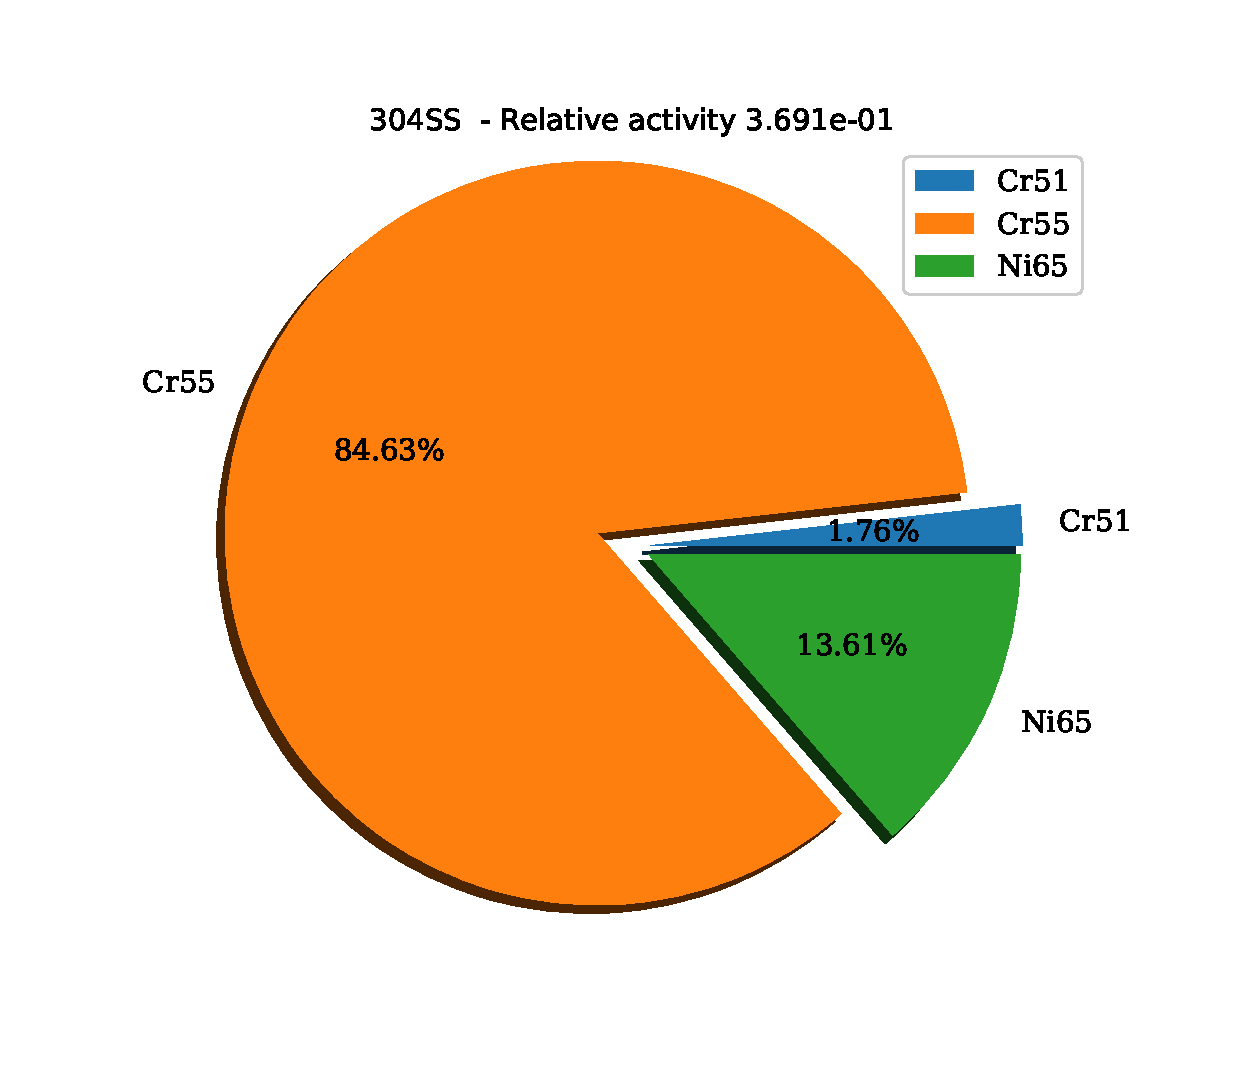
\includegraphics[width=1.0\linewidth]{appendix/pgmactivity/304SS_hot.eps}
\end{minipage}
\begin{minipage}{.49\textwidth}
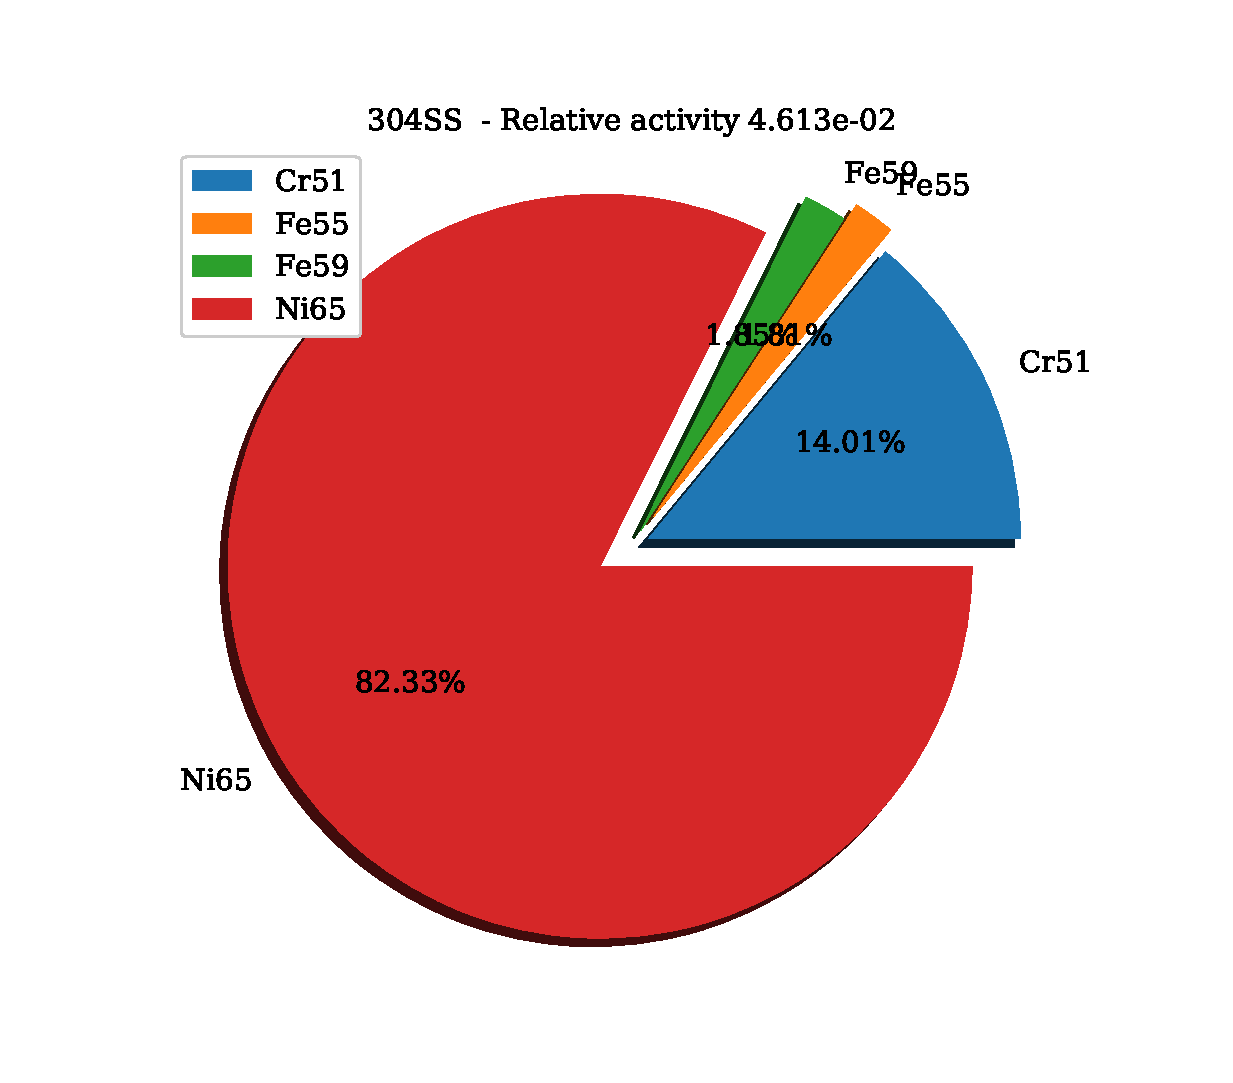
\includegraphics[width=1.0\linewidth]{appendix/pgmactivity/304SS_cooled.eps}
\end{minipage}
\caption{Primary isotopes contributing to activity for plain SS304. Left: hot, right: cooled.}
\label{fig:activity304SS}
\end{figure}


\begin{figure}
\centering
\begin{minipage}{.49\textwidth}
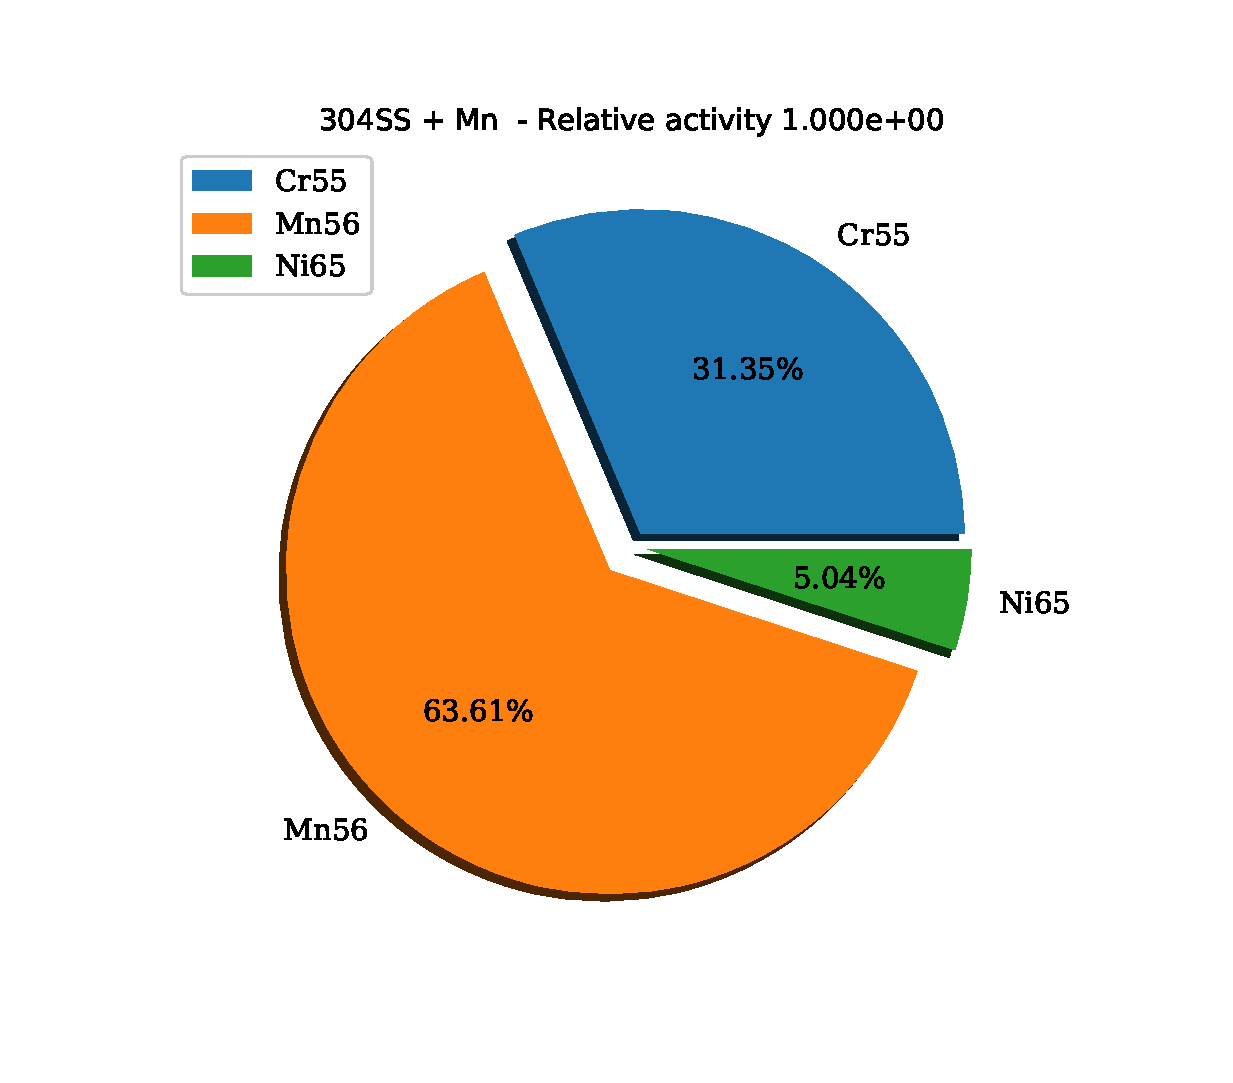
\includegraphics[width=1.0\linewidth]{appendix/pgmactivity/304SS_mn_hot.eps}
\end{minipage}
\begin{minipage}{.49\textwidth}
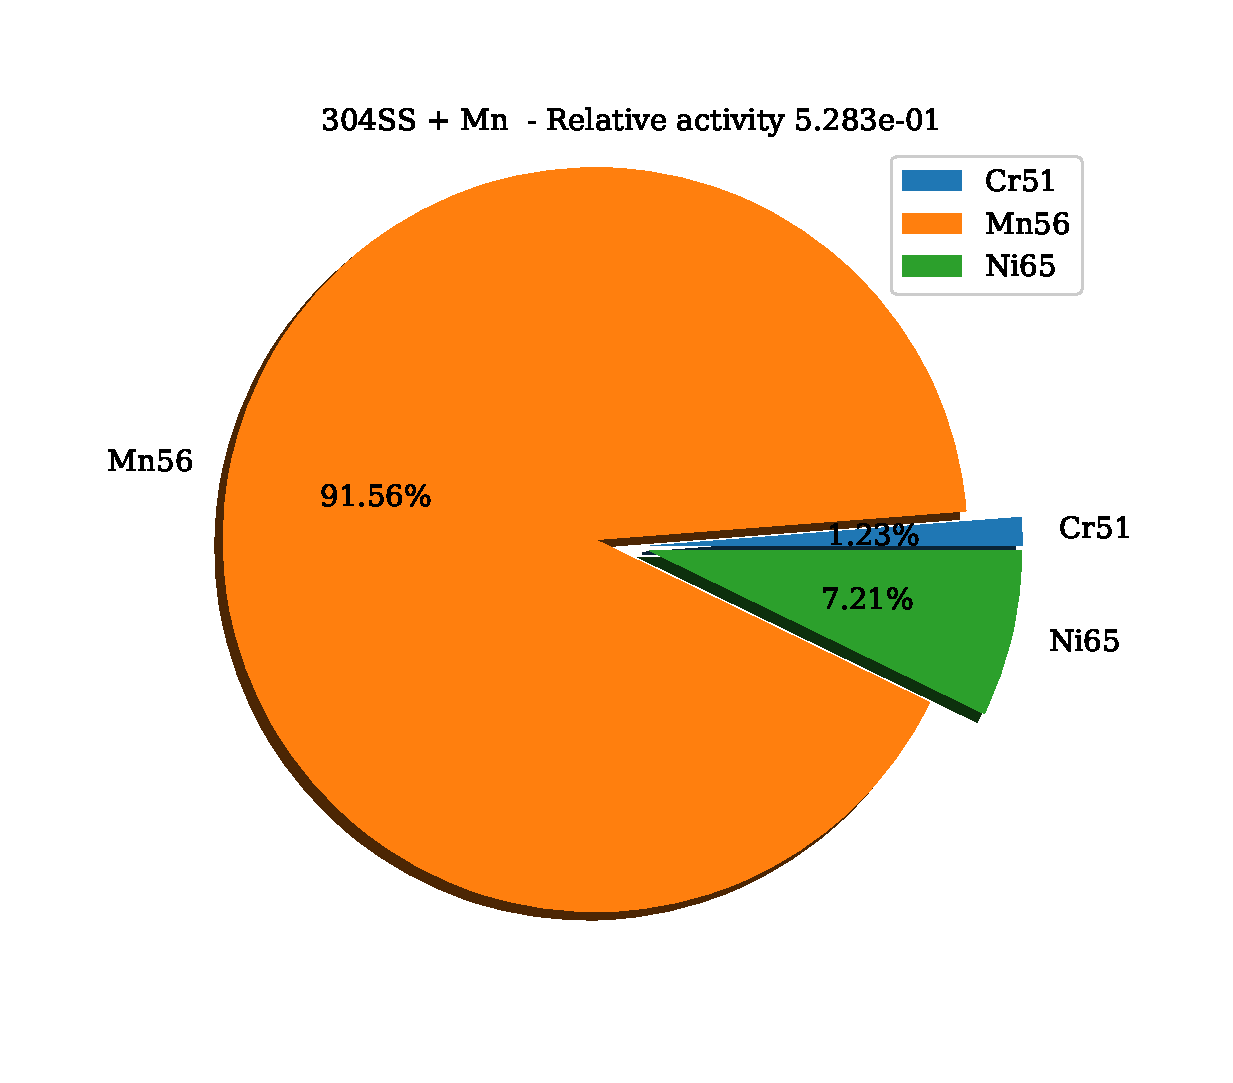
\includegraphics[width=1.0\linewidth]{appendix/pgmactivity/304SS_mn_cooled.eps}
\end{minipage}
\caption{Primary isotopes contributing to activity for SS304 + 1\%Mn. Left: hot, right: cooled.}
\label{fig:activity304SSmn}
\end{figure}

\begin{figure}
\centering
\begin{minipage}{.49\textwidth}
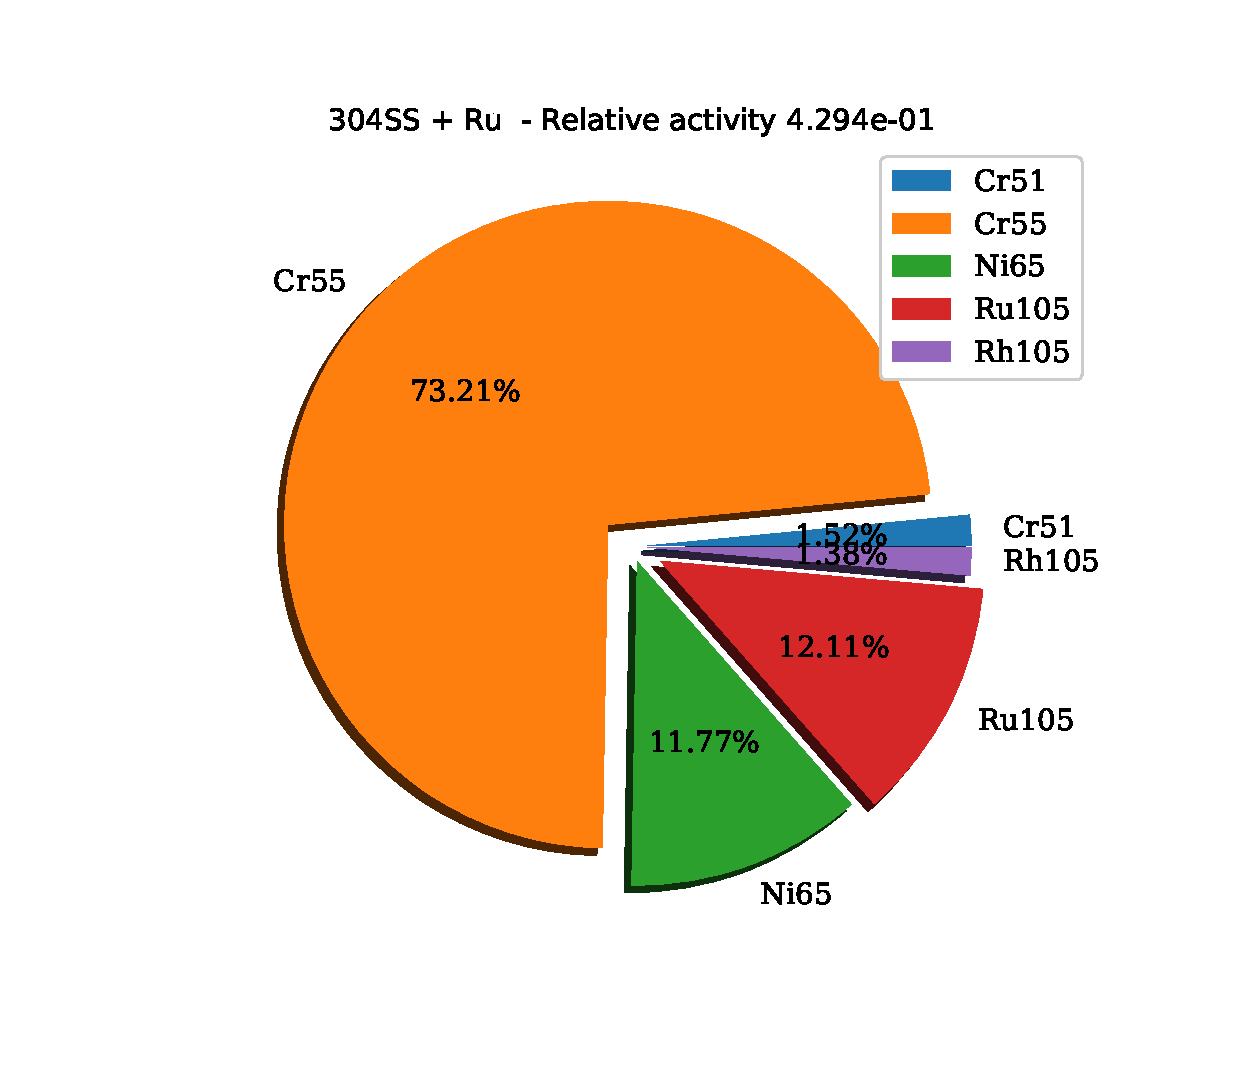
\includegraphics[width=1.0\linewidth]{appendix/pgmactivity/304SS_ru_hot.eps}
\end{minipage}
\begin{minipage}{.49\textwidth}
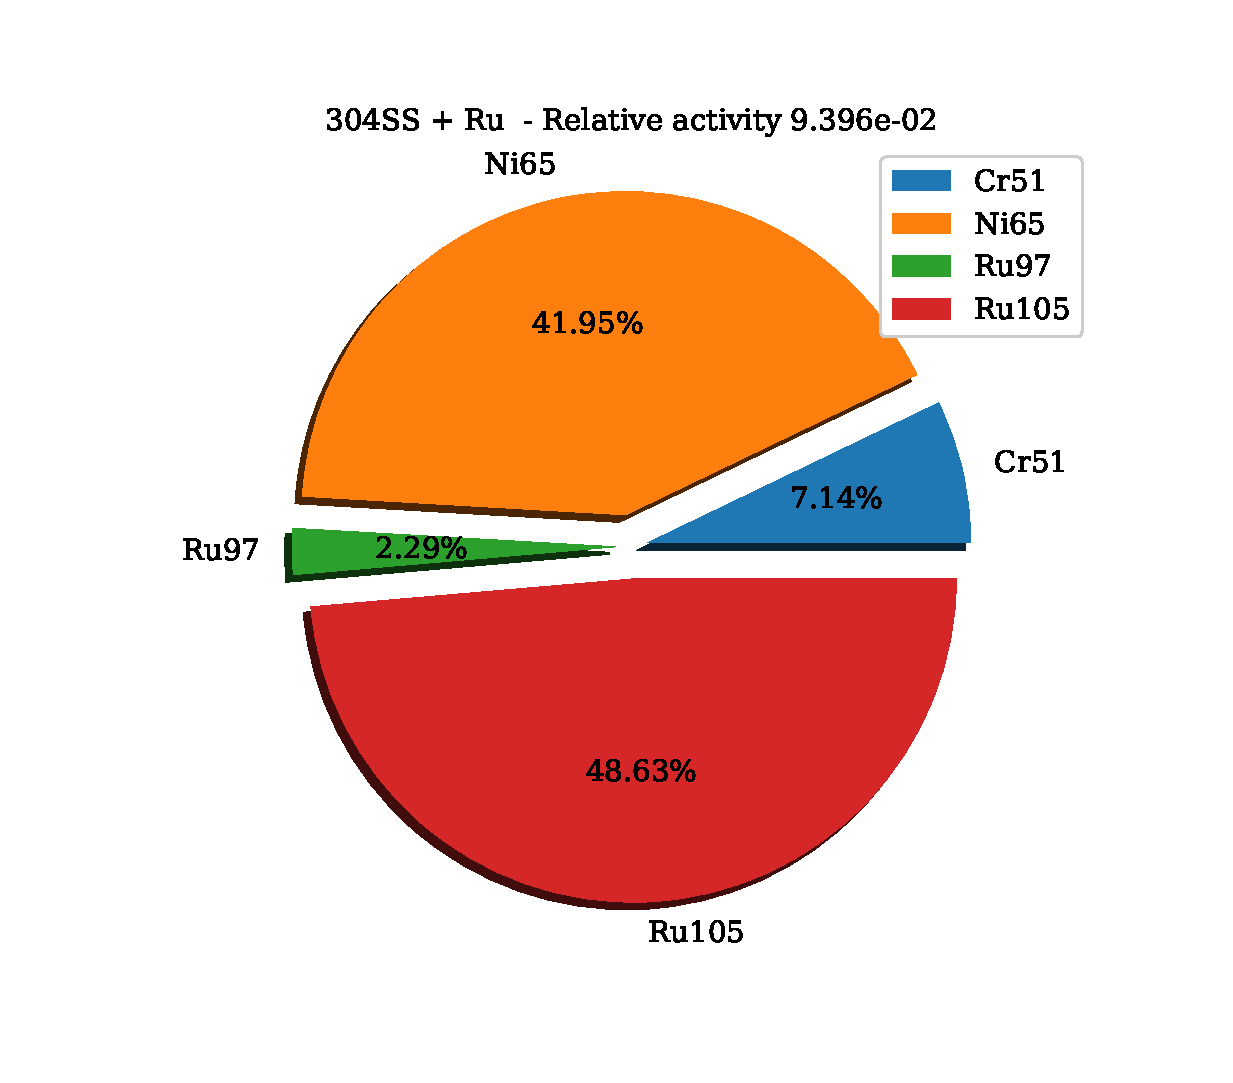
\includegraphics[width=1.0\linewidth]{appendix/pgmactivity/304SS_ru_cooled.eps}
\end{minipage}
\caption{Primary isotopes contributing to activity for SS304 + 1\%Ru. Left: hot, right: cooled.}
\label{fig:activity304SSru}
\end{figure}

\begin{figure}
\centering
\begin{minipage}{.49\textwidth}
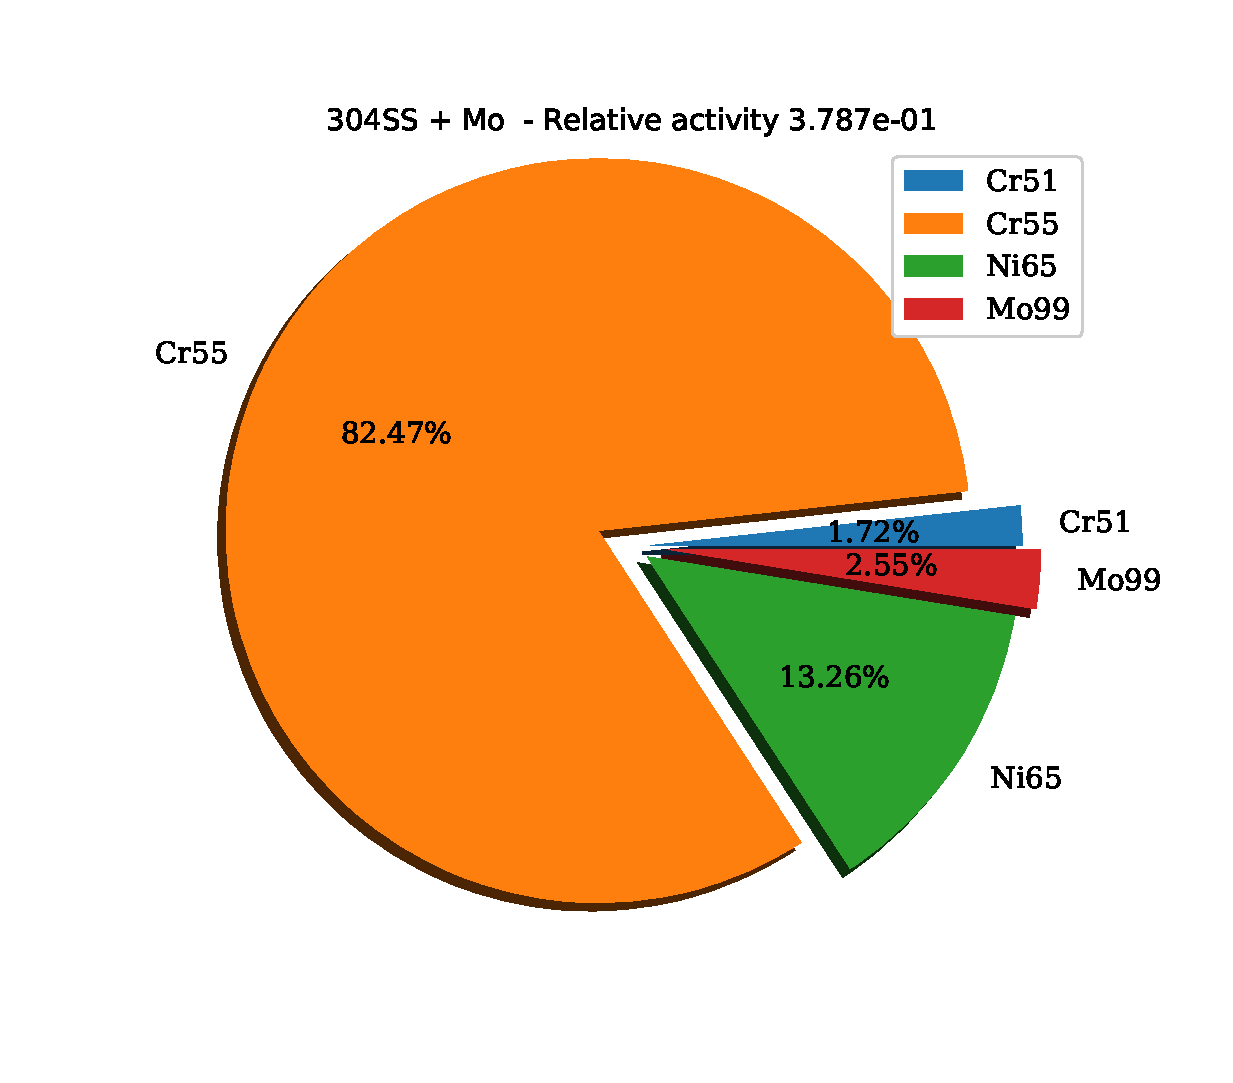
\includegraphics[width=1.0\linewidth]{appendix/pgmactivity/304SS_mo_hot.eps}
\end{minipage}
\begin{minipage}{.49\textwidth}
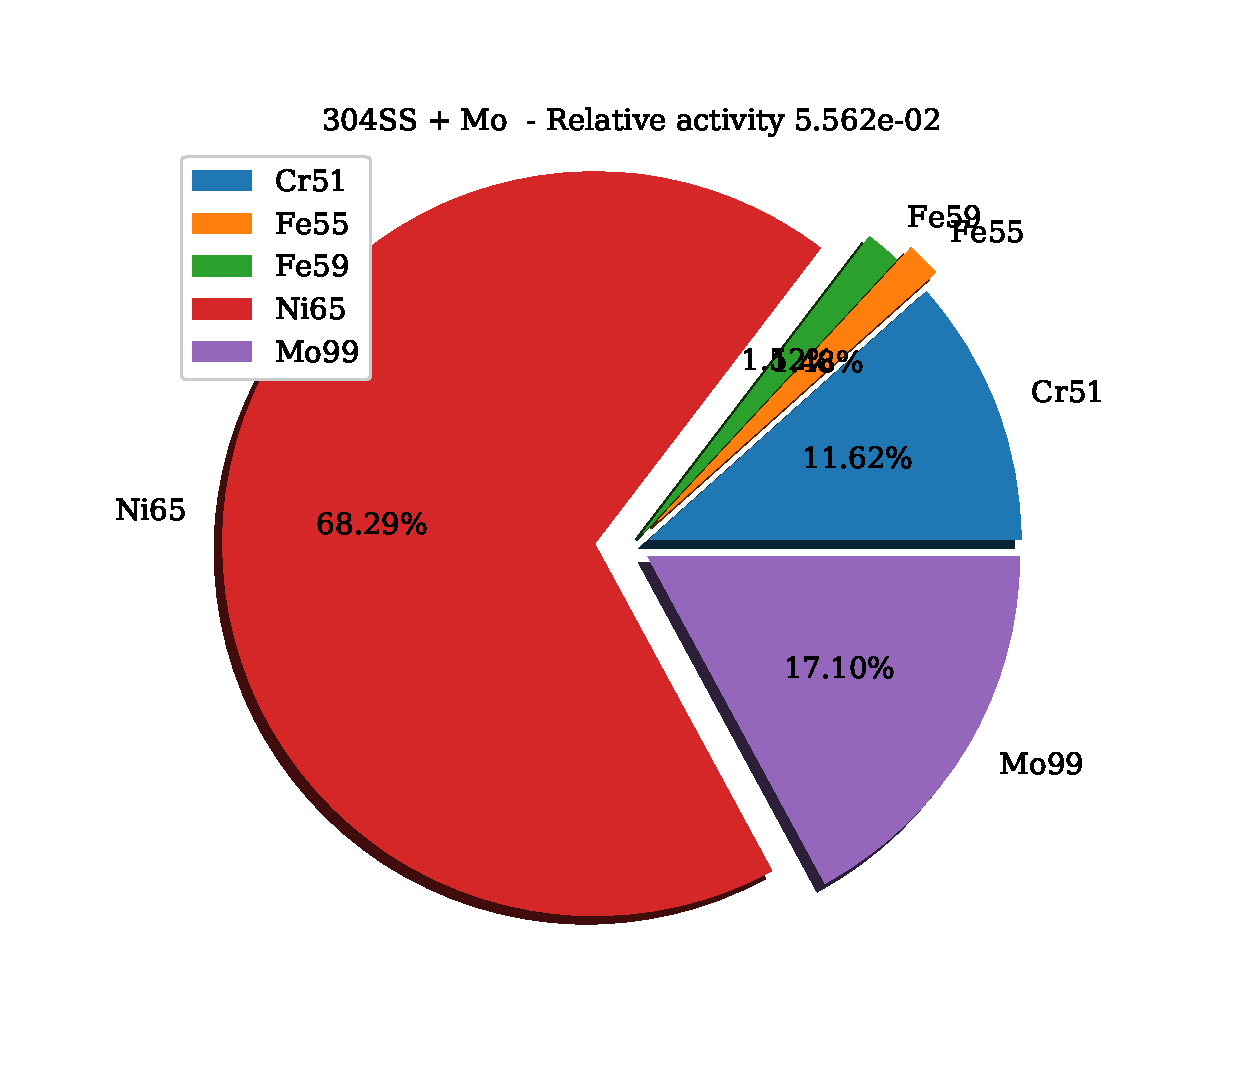
\includegraphics[width=1.0\linewidth]{appendix/pgmactivity/304SS_mo_cooled.eps}
\end{minipage}
\caption{Primary isotopes contributing to activity for SS304 + 1\%Mo. Left: hot, right: cooled.}
\label{fig:activity304SSmo}
\end{figure}

\begin{figure}
\centering
\begin{minipage}{.49\textwidth}
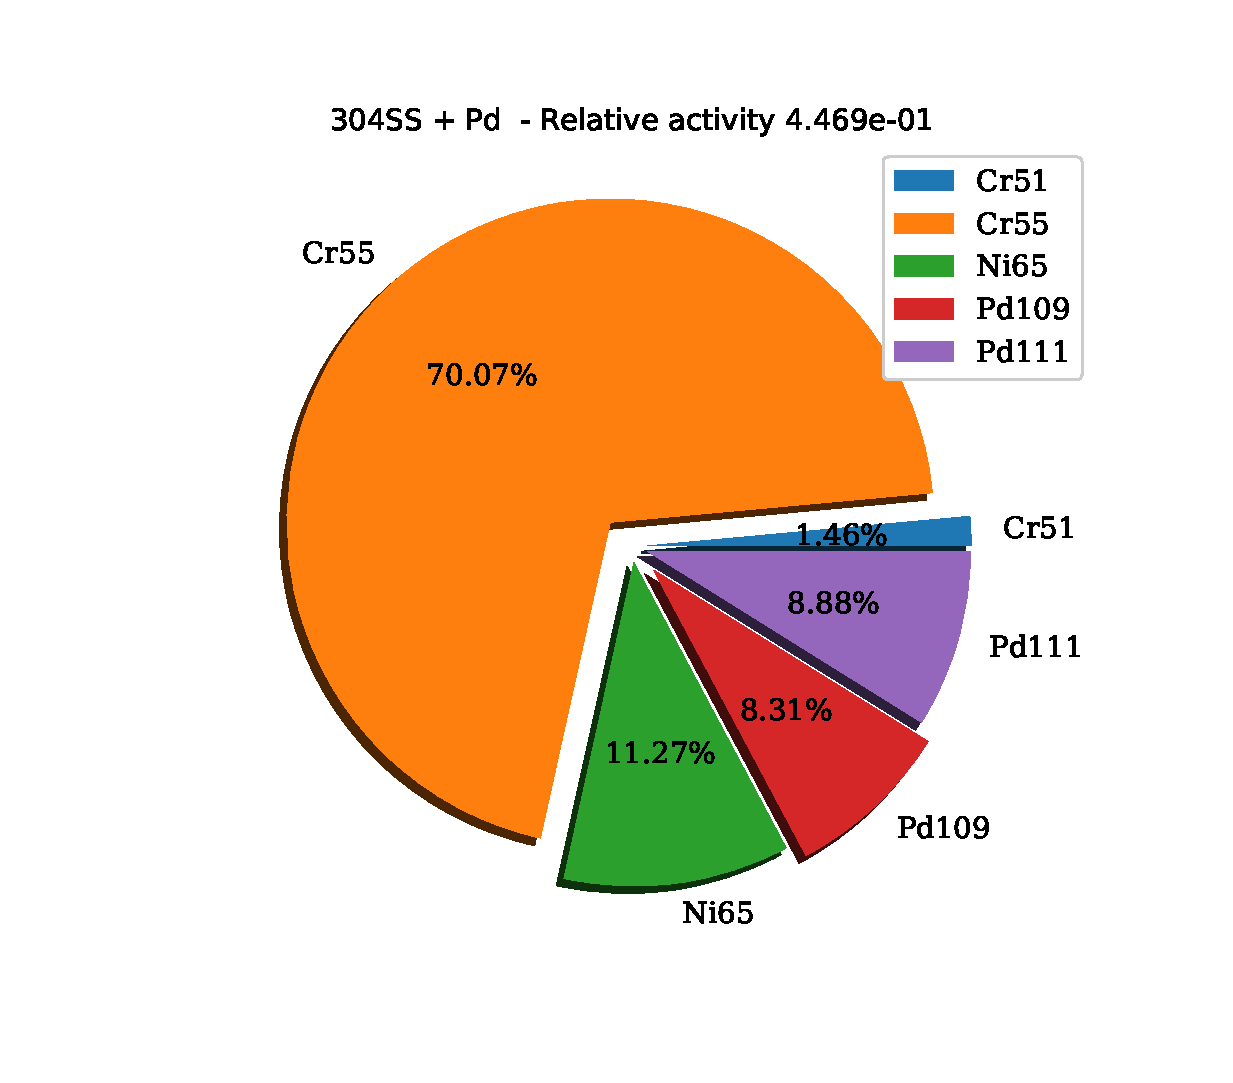
\includegraphics[width=1.0\linewidth]{appendix/pgmactivity/304SS_pd_hot.eps}
\end{minipage}
\begin{minipage}{.49\textwidth}
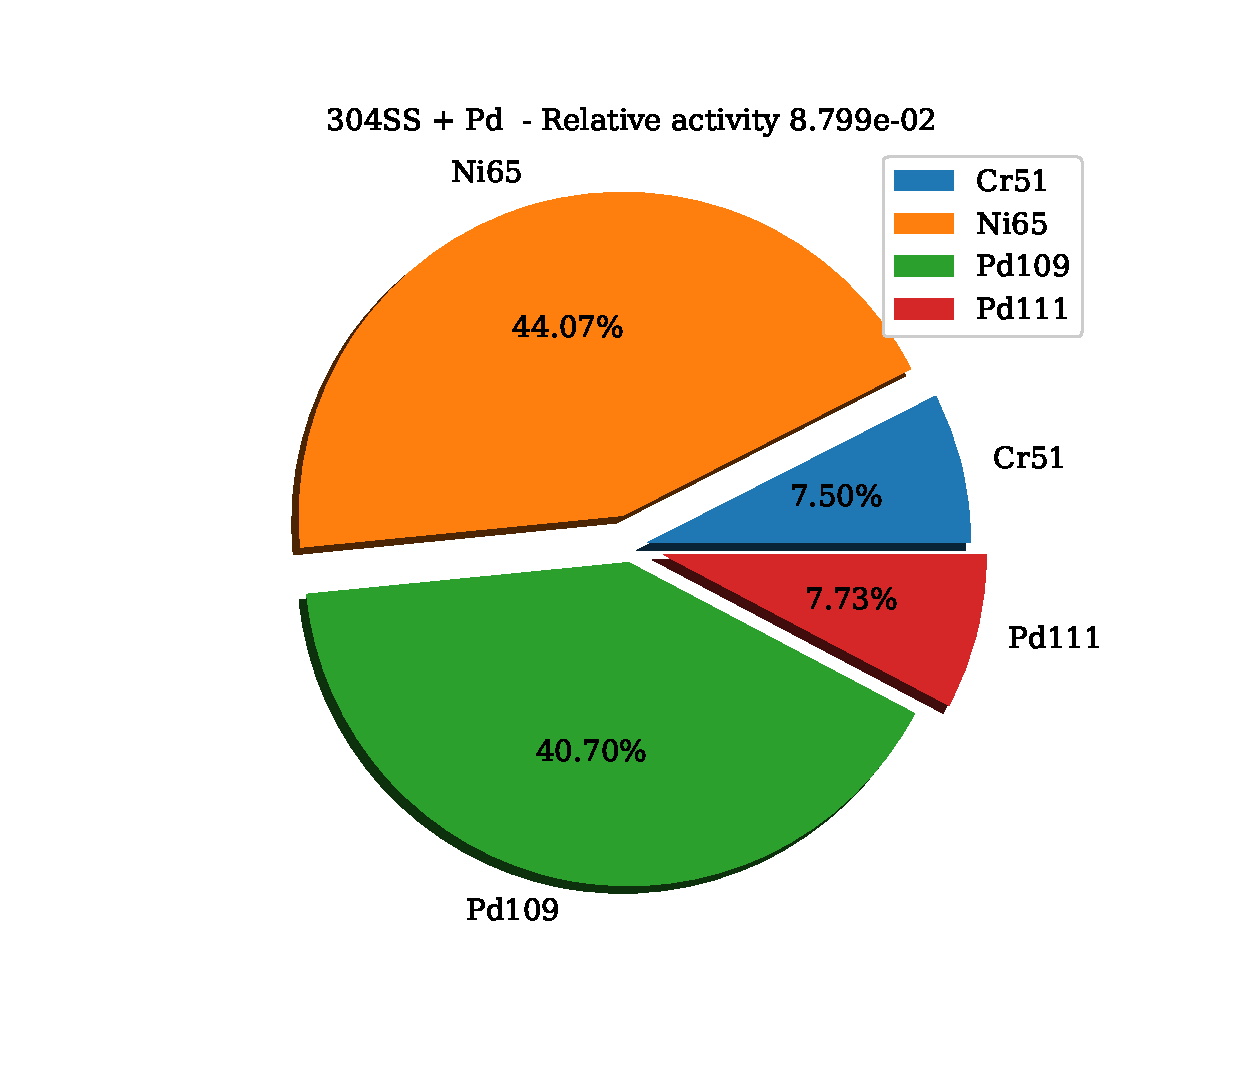
\includegraphics[width=1.0\linewidth]{appendix/pgmactivity/304SS_pd_cooled.eps}
\end{minipage}
\caption{Primary isotopes contributing to activity for SS304 + 1\%Pd. Left: hot, right: cooled.}
\label{fig:activity304SSpd}
\end{figure}

\begin{figure}
\centering
\begin{minipage}{.49\textwidth}
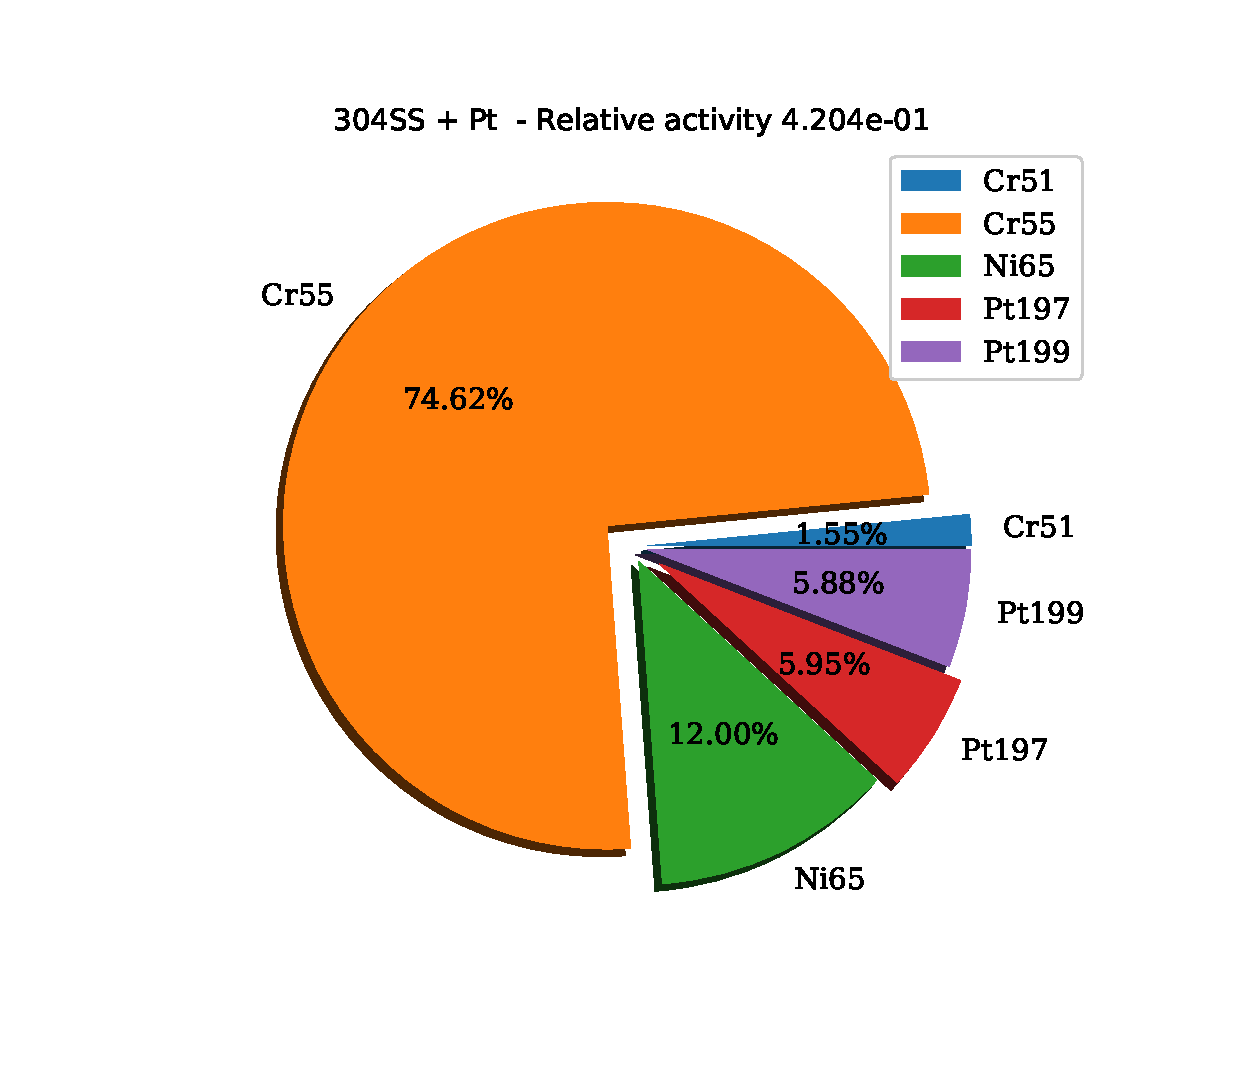
\includegraphics[width=1.0\linewidth]{appendix/pgmactivity/304SS_pt_hot.eps}
\end{minipage}
\begin{minipage}{.49\textwidth}
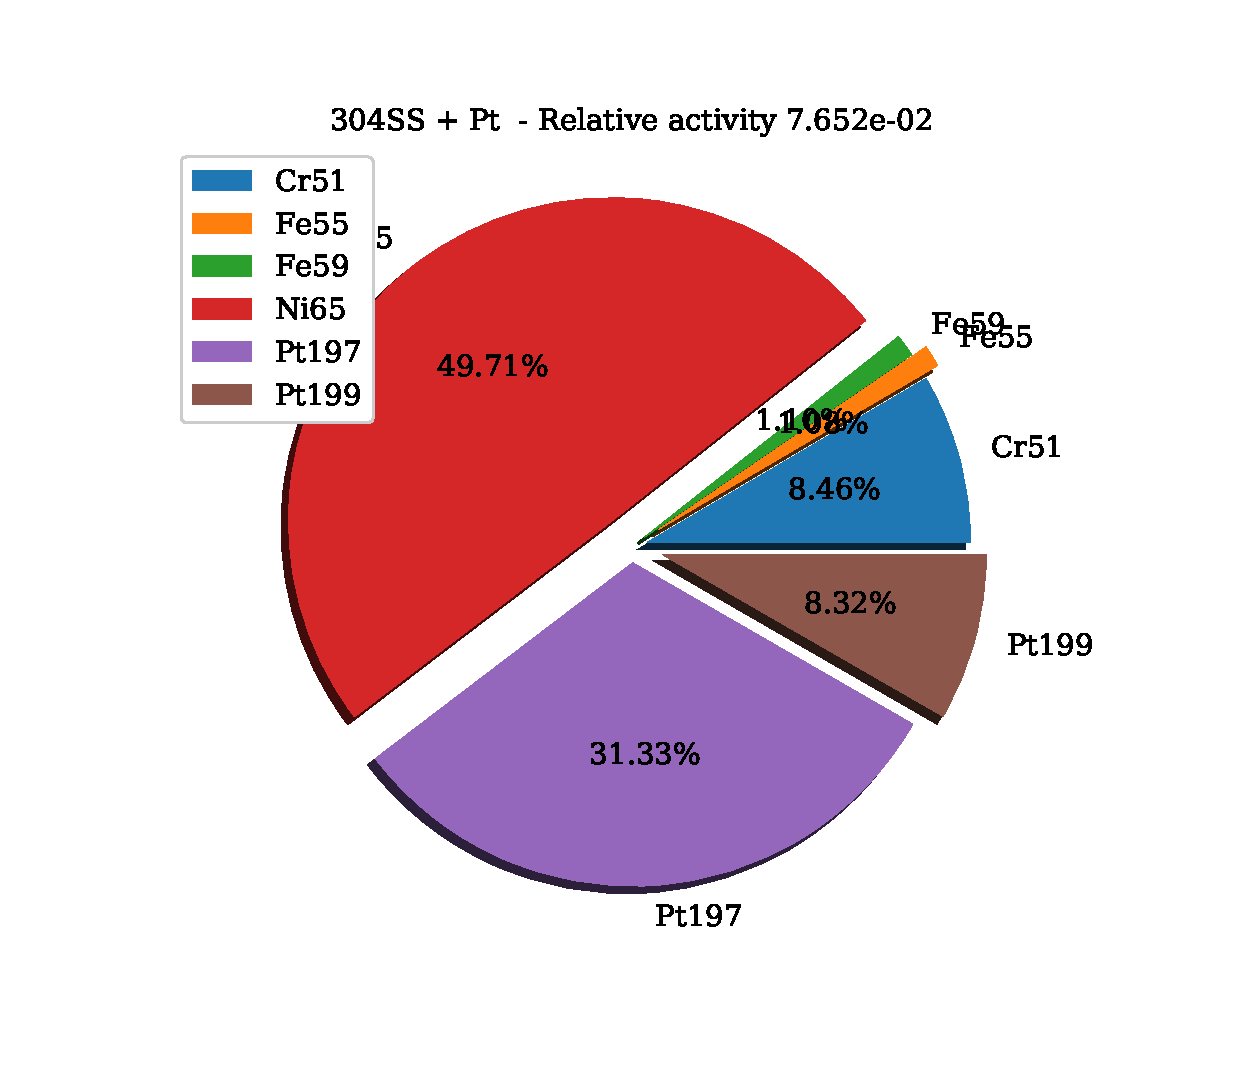
\includegraphics[width=1.0\linewidth]{appendix/pgmactivity/304SS_pt_cooled.eps}
\end{minipage}
\caption{Primary isotopes contributing to activity for SS304 + 1\%Pd. Left: hot, right: cooled.}
\label{fig:activity304SSpt}
\end{figure}


